%%%%%%%%%%%%%%%%%%%%%%%%%%%%%%%%%%%%%%%%%%%%%%%%%%%%%%%%%%%%%%%%%%%%%%%%%%%%%%%%%%%%%%%
%%%%%%%%%%%%%%%%%%%%%%%%%%%%%%%%%%%%%%%%%%%%%%%%%%%%%%%%%%%%%%%%%%%%%%%%%%%%%%%%%%%%%%%
% 
% This top part of the document is called the 'preamble'.  Modify it with caution!
%
% The real document starts below where it says 'The main document starts here'.


\documentclass[12pt]{article}

\usepackage{amssymb,amsmath,amsthm}
\usepackage[top=1in, bottom=1in, left=1.25in, right=1.25in]{geometry}
\usepackage{fancyhdr}
\usepackage{listings}
\usepackage{enumerate}
\usepackage{hieroglf}
\usepackage{oands}
\usepackage{arevmath}
\usepackage{relsize}
\usepackage{times,txfonts}
\usepackage{graphicx}
\usepackage{float}

\newtheoremstyle{homework}% name of the style to be used
  {18pt}% measure of space to leave above the theorem. E.g.: 3pt
  {12pt}% measure of space to leave below the theorem. E.g.: 3pt
  {}% name of font to use in the body of the theorem
  {}% measure of space to indent
  {\bfseries}% name of head font
  {:}% punctuation between head and body
  {2ex}% space after theorem head; " " = normal interword space
  {}% Manually specify head
\theoremstyle{homework} 

% Set up an Exercise environment and a Solution label.
\newtheorem*{exercisecore}{Exercise \@currentlabel}
\newenvironment{exercise}[1]
{\def\@currentlabel{#1}\exercisecore}
{\endexercisecore}

\newcommand{\localhead}[1]{\par\smallskip\noindent\textbf{#1}\nobreak\\}%
\newcommand\solution{\localhead{Solution:}}

%%%%%%%%%%%%%%%%%%%%%%%%%%%%%%%%%%%%%%%%%%%%%%%%%%%%%%%%%%%%%%%%%%%%%%%%
%
% Stuff for getting the name/document date/title across the header
\makeatletter
\RequirePackage{fancyhdr}
\pagestyle{fancy}
\fancyfoot[C]{\ifnum \value{page} > 1\relax\thepage\fi}
\fancyhead[L]{\ifx\@doclabel\@empty\else\@doclabel\fi}
\fancyhead[C]{\ifx\@docdate\@empty\else\@docdate\fi}
\fancyhead[R]{\ifx\@docauthor\@empty\else\@docauthor\fi}
\headheight 15pt

\def\doclabel#1{\gdef\@doclabel{#1}}
\doclabel{Use {\tt\textbackslash doclabel\{MY LABEL\}}.}
\def\docdate#1{\gdef\@docdate{#1}}
\docdate{Use {\tt\textbackslash docdate\{MY DATE\}}.}
\def\docauthor#1{\gdef\@docauthor{#1}}
\docauthor{Use {\tt\textbackslash docauthor\{MY NAME\}}.}
\makeatother

% Shortcuts for blackboard bold number sets (reals, integers, etc.)
\newcommand{\Reals}{\ensuremath{\mathbb R}}
\newcommand{\Nats}{\ensuremath{\mathbb N}}
\newcommand{\Ints}{\ensuremath{\mathbb Z}}
\newcommand{\Rats}{\ensuremath{\mathbb Q}}
\newcommand{\Cplx}{\ensuremath{\mathbb C}}
%% Some equivalents that some people may prefer.
\let\RR\Reals
\let\NN\Nats
\let\II\Ints
\let\CC\Cplx

%%%%%%%%%%%%%%%%%%%%%%%%%%%%%%%%%%%%%%%%%%%%%%%%%%%%%%%%%%%%%%%%%%%%%%%%%%%%%%%%%%%%%%%
%%%%%%%%%%%%%%%%%%%%%%%%%%%%%%%%%%%%%%%%%%%%%%%%%%%%%%%%%%%%%%%%%%%%%%%%%%%%%%%%%%%%%%%
% 
% The main document start here.

% The following commands set up the material that appears in the header.
\doclabel{Math 316: HW 6}
\docauthor{Stefano Fochesatto}
\docdate{\today}

\begin{document}


\textbf{Section 5.3}

\begin{exercise}{21} Bhaskara, 1150. What number divided by 6 leaves a remainder of 5, divided by 5
  leaves a remainder of 4, divided by 4 leaves a remainder of 3, and divided by 3 leaves a remainder of 2? Written in our modern notation, solve for $N$ such that,
  \begin{align*}
    N &\cong 5 mod 6,\\
    N &\cong 4 mod 5,\\
    N &\cong 3 mod 4,\\
    N &\cong 2 mod 3.
  \end{align*}
  \solution By definition we know that $6,5,4,3|(N + 1)$, since if we were to add one to $N$, the remainders would all increase by one 
  and become the size of the moduli. Thus all solutions are a multiple of $6,5,4$ and $3$ minus $1$,
  \begin{equation*}
    N = LCM(6,5,4,3)k - 1 
  \end{equation*}
  for some $k \in \Nats$.
  I like the prime factorization method of finding the LCM so listing the prime factorization,
  \begin{align*}
    3 &= 3,\\
    4 &= 2^2,\\
    5 &= 5,\\
    6 &= 2(3).\\
  \end{align*} 
Solving for the LCM as the product of the maximum occurrence of each prime, 
\begin{equation*}
  LCM(6,5,4,3) = 2^2(3)(5) = 60.
\end{equation*}
So we get that for all $k \in \Nats$,
\begin{equation*}
  N = 60k - 1.
\end{equation*}
\end{exercise}
\vspace{.5in}


\textbf{Section 5.5}

\begin{exercise}{1} Solve the following quadratic equations with the arabic method of complete the square.\\
  \begin{enumerate}
    \item $x^2 + 12x = 64$\\
    \solution First note that this is a type 4 problem with the form $ax^2 + bx = 2$. We complete the square by noting that, 
    \begin{equation*}
      (x + 6)^2 = x^2 + 12x + 36. 
    \end{equation*}
    So adding 36 to both sides we get that,
    \begin{align*}
      x^2 + 12x + 36 &= 64 + 36,\\
      (x + 6)^2 &= 100,\\
      (x + 6)^2 &= 10^2.
    \end{align*}
    Therefore $x = 4, -12$. 




    \vspace{.25in}

    \item $3x^2 + 10x = 32$\\
    \solution From the hint lets multiply both sides of the equation by 3 and and simplify the form of our equation with a substitution of $y = 3x$, 
    \begin{align*}
      3x^2 + 10x &= 32,\\
      3(3x^2 + 10x) &= 3(32),\\
      9x^2 + 30x &= 96,\\
      (3x)^2 + 10(3x) &= 96,\\
      (y)^2 + 10(y) &= 96.
    \end{align*}
    Now our problem is a type 4 problem with the form $ax^2 + bx = 2$. We complete the square by noting that, 
    \begin{equation*}
      (y + 5)^2 = y^2 + 10y + 25. 
    \end{equation*}
    So adding 25 to both sides, 
    \begin{align*}
      y^2 + 10y + 25 &= 96 + 25,\\
      (y + 5)^2 &= 121,\\
      (y + 5)^2 &= (11)^2.
    \end{align*}
    Thus we get that $y = 6, -16$ and since $y = 3x$ we get that $x = 2, \frac{-16}{3}$
    \vspace{.25in}


  \end{enumerate}
\end{exercise}
\vspace{.5in}

\begin{exercise}{7}
  \begin{enumerate}
    \item Show that the cubic equation $x^3 + b^2c = b^2x$ can be solved by finding the intersection of the 
    parabola $x^2 = by$ and the hyperbola $y^2 + cx = x^2$.\\

    \solution We can show that the intersection of $x^2 = by$ and $y^2 + cx = x^2$ gives $x^3 + b^2c = b^2x$ through algebra.
    First solve the first equation for $y$, 
    \begin{equation*}
      y = \frac{x^2}{b}. 
    \end{equation*}
    Now substituting into the second equation and doing some algebra to get the third equation. 
    \begin{align*}
      (\frac{x^2}{b})^2 + cx &= x^2,\\
      \frac{x^4}{b^2} + cx &= x^2,\\
      \frac{x^4}{b^2} + cx &= x^2,\\
      \frac{x^3}{b^2} + c &= x,\\
      x^3 + b^2c &= b^2x.\\
    \end{align*}
    Therefore where the two conic sections intersect we get the solution to the cubic. 
  \begin{center}
    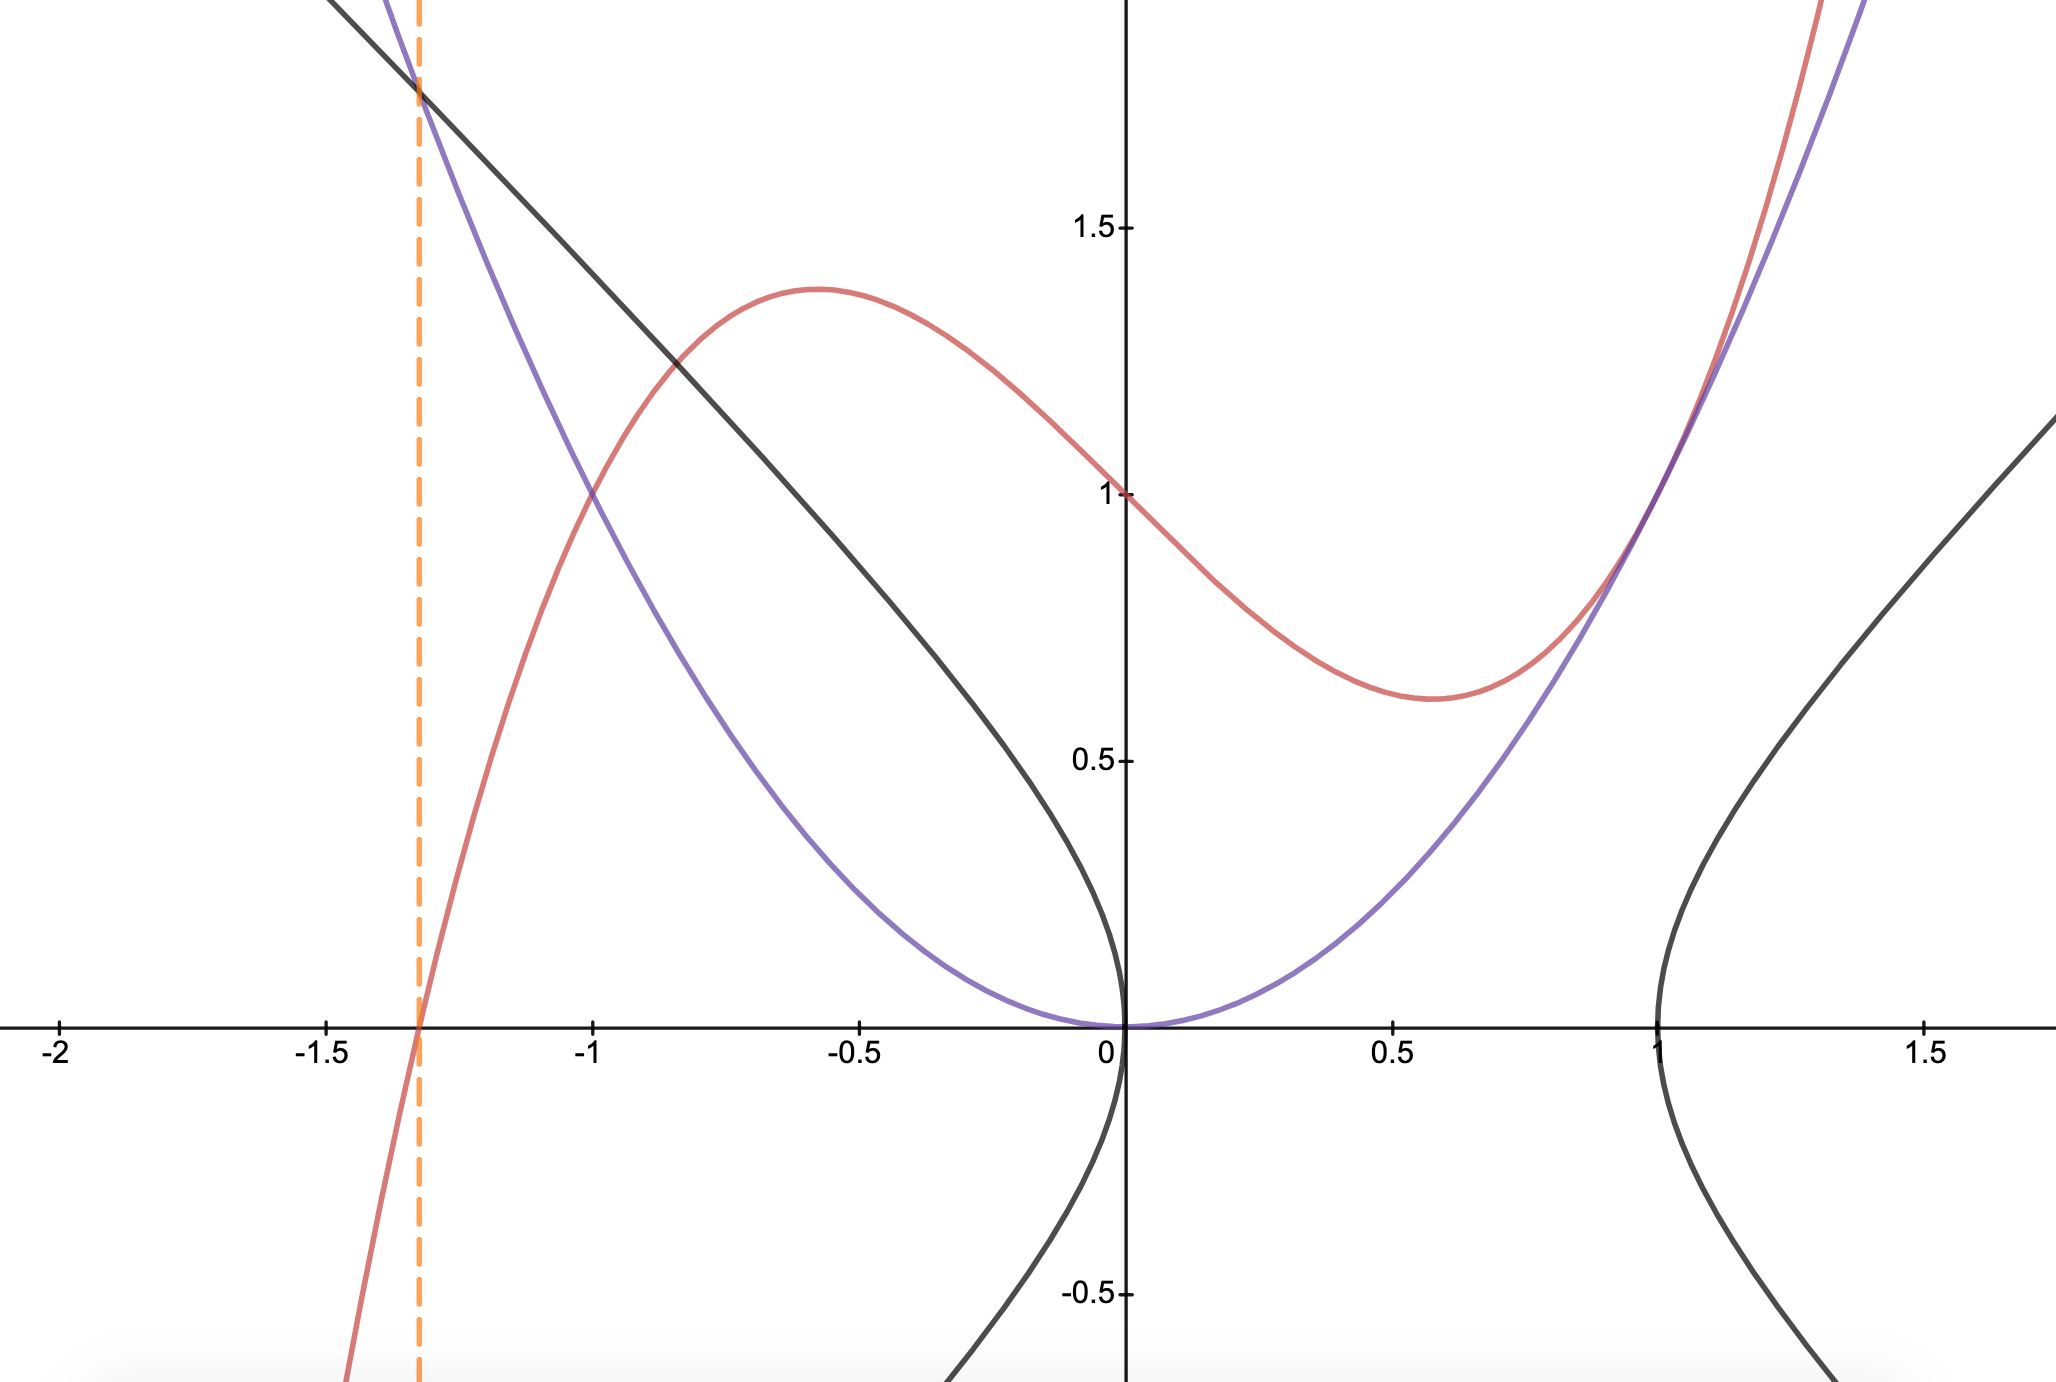
\includegraphics[width = .90\textwidth]{curve1.png}
  \end{center}  




    \vspace{.25in}


    \item Show that the cubic equation $x^3 + c = ax^2$ can be solved by finding the intersection of the parabola $y^2 + cx = ac$
    and the rectangular hyperbola $xy = c$. \\

    \solution Again we can show this through algebra. Solving the rectangular hyperbola for $y$,
    \begin{equation*}
      y = \frac{c}{x}.
    \end{equation*}
    Substotutinog into the parabola and doing some algebra to get the cubic,
    \begin{align*}
      y^2 + cx &= ac,\\
      (\frac{c}{x})^2 + cx &= ac,\\
      \frac{c^2}{x^2} + cx &= ac,\\
      c^2 + cx^3 &= acx^2,\\
      c + x^3 &= ax^2,\\
      x^3 + c &= ax^2.
    \end{align*}
    Thus where the two conic sections intersect we get the solution to the cubic. 

    
  \begin{center}
    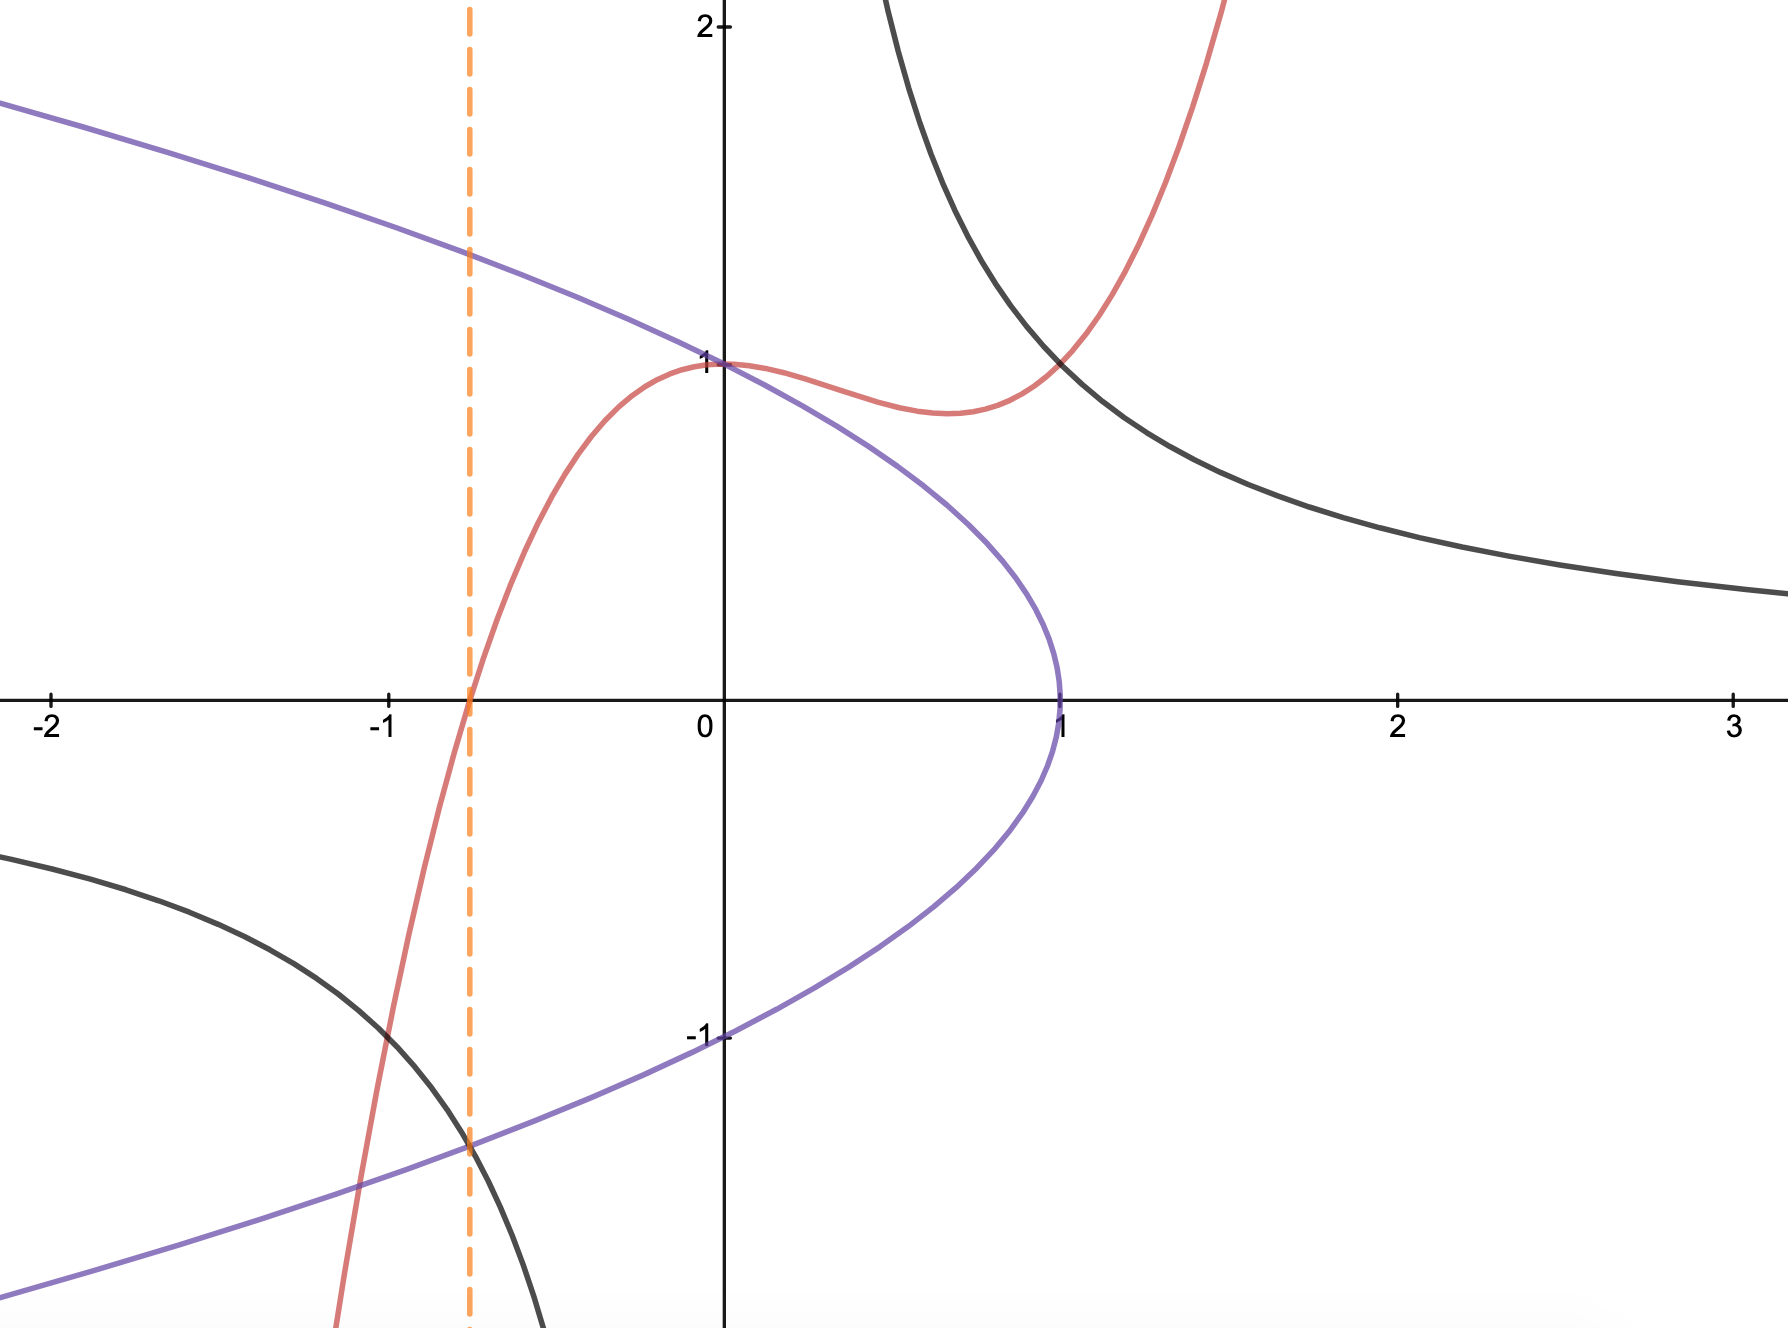
\includegraphics[width = .90\textwidth]{curve2.png}
  \end{center}  

  \end{enumerate}
\end{exercise}
\vspace{.5in}

\textbf{Additional Problems}

\begin{exercise}{1} Use GeoGebra to verify brahmagupta's result on cyclic quadrilaterals, that is if $\square ABCD$ is a cyclic 
  quadrilateral (all points on a single circle), then
  \begin{equation*}
    Area(ABCD) = \sqrt{(s - a)(s - b)(s - c)(s - d)},
  \end{equation*}
  where $s = \frac{1}{2}(a+b+c+d)$. To verify, construct a working diagram in GeoGebra, measure the appropriate quantities, calculate the appropriate
  calculations, and then show me two snapshots with different placements of $A,B,C,D$ on the circle where I can see the equal quantities.\\ 

  \solution We begin our GeoGebra construction by drawing a circle with origin $O$ and then a line $DC$ which intersect the circle in two places like a chord.
  From there we create two more lines, one that starts at $D$ and intersects the circle at $A$ and another that starts at $C$ intersecting the circle at 
  $B$. Using the GeoGebra console we can display the lengths of the quadrilateral, calculate $s$, the area $l$, and Brahmagupta's result.
  
  \begin{center}
    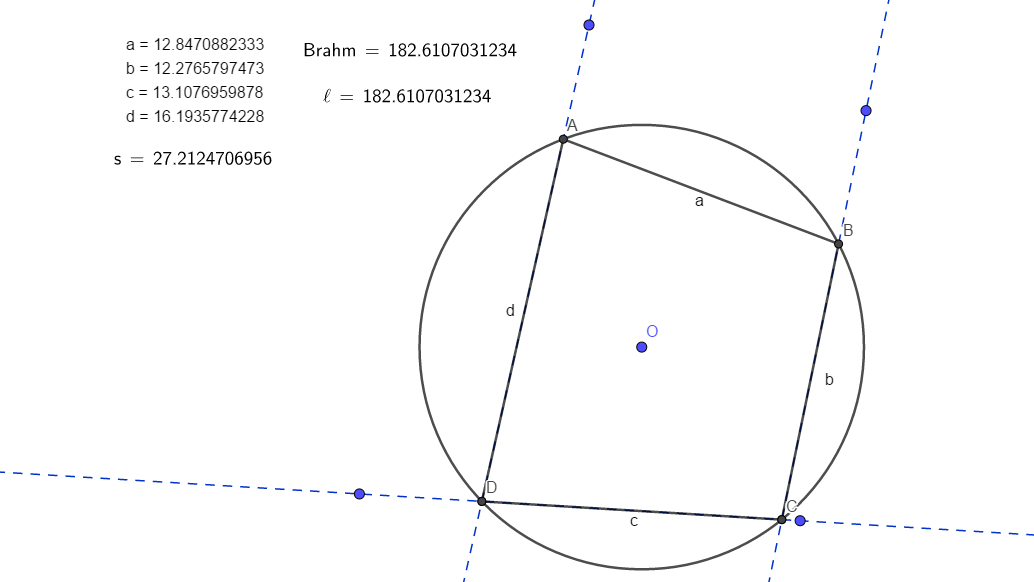
\includegraphics[width = \textwidth]{bram1.png}
  \end{center}  
  \vspace{.15in}


  \begin{center}
    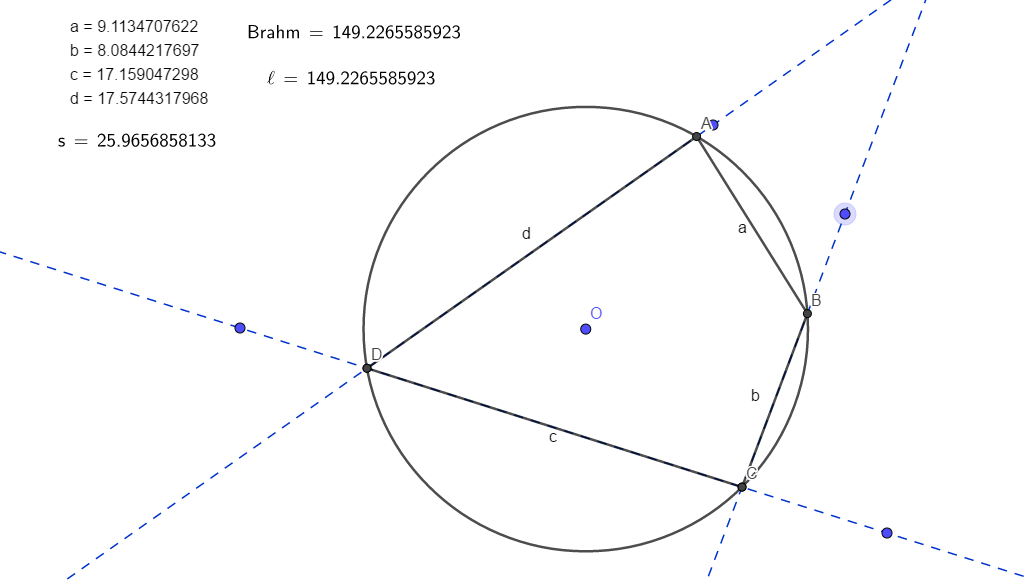
\includegraphics[width = \textwidth]{bram2.png}
  \end{center}  

\end{exercise}
\vspace{.5in}


\begin{exercise}{2}Al-Khwarizimi gives the following rule for his sixth case, $bx + c = x^2$ (recall the "root"
  or "number of roots" is the coefficients of the $x$ term and the "number" is the constant term):\\

  \indent \textit{Halve the number of roots. Multiply this by itself. Add this square to the number. Extract the square root. Add this to half of the 
  number of roots. that is the solution.}\\

  \begin{enumerate}
    \item Translate this into a formula using $x, b, c$.\\
    \solution Following the description we know that the solution of the quadratic is $x$ and we will start by halving the number
    of roots $(b)$ and then squaring that result,
    \begin{equation*}
      x = (\frac{b}{2})^2.
    \end{equation*}
    Adding this result to the number $(c)$ and then square rooting we get,
    \begin{equation*}
      x = \sqrt{(\frac{b}{2})^2 + c}.
    \end{equation*}
    Finally we add half the number of roots $(b)$,
    \begin{equation*}
      x = \sqrt{(\frac{b}{2})^2 + c} + \frac{b}{2}.
    \end{equation*}  
    \vspace{.25in}

    \item Give a geometric argument for its validity using the following diagram where $c$ is the area of the gray rectangle
    $ABCD$ , $AE = EF = x$, $FC = b$, $M$ is the midpoint of $FC$, and every angle is orthogonal.\\
    \begin{center}
      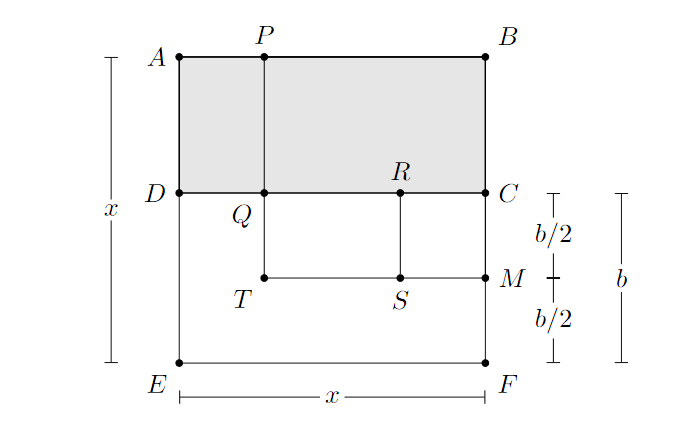
\includegraphics[width = .75\textwidth]{quadratic.png}
    \end{center}  
    \solution First note that $area(\square RCMS) = (\frac{b}{2})^2$, and that $\square DAPQ \cong \square TQRS$(must show $DQ = \frac{b}{2}$ or $TS = x - b$).
    So finally we ge that the $area(\square PBMT) = c + (\frac{b}{2})^2$ where the side length is $x - \frac{b}{2}$. So,
    \begin{equation*}
      \sqrt{(\frac{b}{2})^2 + c} + \frac{b}{2} = \sqrt{area(\square PBMT)} + \frac{b}{2} = x - \frac{b}{2} + \frac{b}{2} = x.
    \end{equation*}  


  \end{enumerate}


\end{exercise} 
\vspace{.5in}


\textbf{Reflection}
\begin{enumerate}
  \item I found the first problem was difficult to do in anyway that was explained in the book. I tried the "finding one" method but it doesn't
  work if your moduli are not relatively prime. I ended up solving it with a more modern method. \\
  
  \item I don't see how we can show that  $DQ = \frac{b}{2}$ or $TS = x - b$ in the last problem, but I definitely see how you could get the formula from the diagram. 

\end{enumerate}








\end{document}